\section{Lösungsidee}
Um möglichst effizient Kreismittelpunkte zu bestimmen mache ich mir zunächst folgende Eigenschaft von Kreisen zunutze: Am Mittelpunkt eines Kreises ist der Abstand (Radius) zu der äußeren Linie des Kreises in jede Richtung gleich (s. Grafik).

\begin{figure}[!ht]
	\centering	
	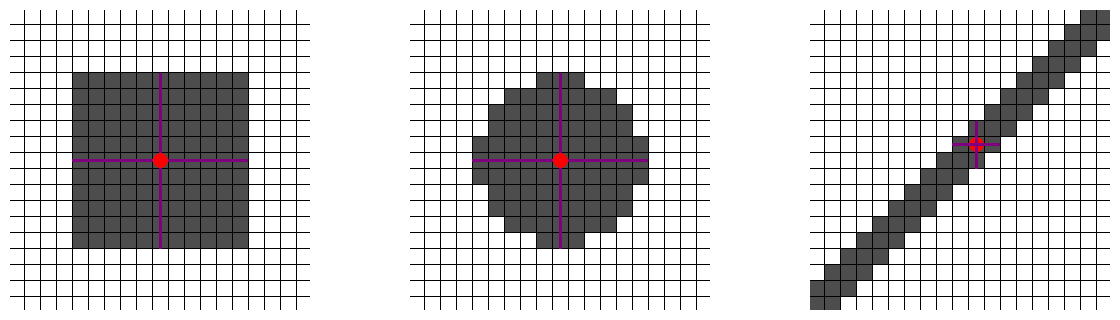
\includegraphics[width=0.8\textwidth]{durchmesservergleich}
	\label{Verschiedene Formen mit eingezeichnetem Mittelpunkt nach erstem Kriterium}
\end{figure}

In einem Bild lassen sich solche Punkte finden, indem man von jedem schwarzen Bildpunkt den Abstand in vertikale wie horizontale Richtung misst und miteineander vergleicht. Von einem Vergleich des Abstandes in andere Richtungen (z.B. diagonal) sollte man bei einem Bild aus Pixeln absehen, da bei der Speicherung eines Kreises als Bitmap aus quadratischen Pixeln diagonale Messungen oder gar Messungen unter beliebigem Winkel falsche Ergebnisse liefern.

Da diese Bedingung jedoch auch Punkte in Quadraten und anderen unregelmäßigen Formen liefert, muss für eine zuverlässige Erkennung eine zweite Eigenschaft von Kreisen genutzt werden: Bei bekannten Durchmesser kann die Fläche eines Kreises mit der Kreisformel bestimmt werden. Diese Soll-Fläche kann mit der tatsächlichen Fläche verglichen werden. Sollte das Delta zwischen diesen beiden Flächengrößen nahe 0 sein, handelt es sich mit großer Wahrscheinlichkeit um einen Kreismittelpunkt.

Danach gilt es noch zu bestimmen ob es sich bei dem Kreis um einen Mittelpunkt eines \task{}s handelt, schließlich sollen sonstige Kreise im Bild nicht ausgegeben werden. Hierzu können wir uns die Proportionen eines \task{s} zu nutze machen: Nach der Kreisaußenseite folgt ein leerer Raum mit der Länge von 1/3 d, gefolgt von einer ebensolangen durchgehend schwarzen Stelle. Ob diese Bedingungen ebenfalls erfüllt sind, lässt sich mit großer Schwierigkeit ermitteln, indem diese Bedingungen vom Mittelpunkt ausgehend rehcts, links, oben und unten prüft. Diagionale und beliebigwinklige Messungen sind nur schwer möglich.

\textbf{Idee: Nochmal so eine coole FloodFill um die Jurorenzu beeindrucken oso}
\section{Umsetzung}
Zunächst überlegte ich mir eine möglichst effiziente Datenstruktur für Grafiken, da die Interaktion über ImageIO mit Bitmaps nicht sonderlich effizient ist. Da für die Erkennung von Kreisen in einer Grafik genaue Informationen über die Farbe eines Bildpunktes nicht relevant sind, kann das Bild beim Einlesevorgang in ein boolesches 2D-Array überführt werden: In diesem Array, das die gleiche Größe wie das eingelesene Bild besitzt, sind die Bildpunkte als True gespeichert, die Teil eines \task sein könnten. In der in Teilaufgabe 1 gegebenen Schwarz-Weiß-Grafik ist diese Einstufung noch simpel: Schwarze Bildpunkte können Teil eines \task sein, sonstige nicht.

Um darauf die Punkte zu bestimmen, deren Radiusse sich in alle vier Richtungen gleichen, muss zunächst die Länge von aufeinanderfolgenden Streifen aus möglichen \task{}-Feldern ermittelt werden. Diese nenne ich nun lineare Zusammenhängigkeitskomponenten. In seperaten Arrays für horizontale und vertikale Streifen speichere ich für jedes Feld die Länge seiner linearen Zusammenhängikeitskomponente. Für ein mögliches \task{}-Feld liegt diese für horizontale Zusmmenhängikeitskomponenten bei
% 1 <= l <= breite
, für vertikale entsprechend bei
% 1 <= l <= höhe
. Bei allen Feldern, die sicher kein Teil eines \task{}s sind, liegt dieser Wert bei 0. 

Danach kann für jede Koordinate die horizontale und vertikale Zusammenhängigkeitskomponentenlänge verglichen werden. Gleichen sie sich, handelt es sich um einen möglichen Mittelpunkt.

Danach kann die Soll-Fläche mit der Kreisformel entweder mit der horizontalen oder vertikalen Zusammenhängigkeitskomponentenlänge berechnet werden. Die tatsächliche Länge kann mit einer Flood-Fill ermittelt werden.

% TODO: Mehrere Punkte wegen kack Anti-Aliasing
\section{Beispiele}
